\section{连接杆零件图制作}
\subsection{生成主视图}
\begin{procedure}
\item 保存连接杆三维模型副本

将构建好的连接杆三维模型另存为“连接杆视图布局.dwg”。

\item 切换至图纸空间

点击命令窗口上面的【布局1】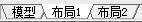
\includegraphics[scale=0.6]{bujukongjian.png} 标签,进入图纸空间。

\item 修改页面设置

调用页面设置管理器,弹出页面设置对话框,将打印机绘图设备修改为“DWG TO PDF.pc3”,图纸尺寸设置为ISO A4(210.00x297.00毫米),设置结果如图\ref{fig:lianjieganpagesetup} 所示。完成后单击图\ref{fig:lianjieganpagesetup}中打印机绘图设备旁边的特性按钮,弹出图\ref{fig:huituyishezhi}所示的绘图仪配置编辑器,选择“设备和文档设置”选项卡中的“修改标准图纸尺寸(可打印区域)”列表,在“修改标准图纸尺寸”对话框中选中ISO full bleed A4(210x297毫米),然后点击修改按钮,弹出\ref{fig:kedayinqushezhi}所示可打印区域设置对话框,并按表\ref{tab:tuzhifumian}尺寸设置可打印区域的值。完成设置后,图纸的幅面和可打印区域均符合图家制图的标准要求。

\begin{figure}[htbp]
\centering
\begin{floatrow}[3]
\ffigbox{\caption{面页设置}\label{fig:lianjieganpagesetup}}{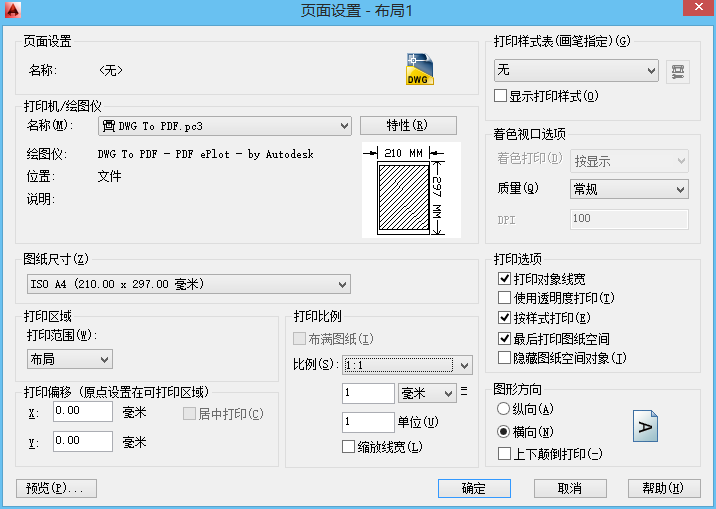
\includegraphics[scale=0.2]{pagesetupdetail.png}}
\ffigbox{\caption{绘图仪配置编辑器}\label{fig:huituyishezhi}}{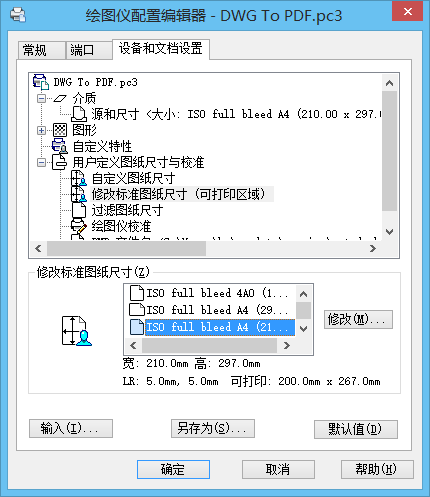
\includegraphics[scale=0.2]{huituyishezhi.png}}
\ffigbox{\caption{可打印区域设置}\label{fig:kedayinqushezhi}}{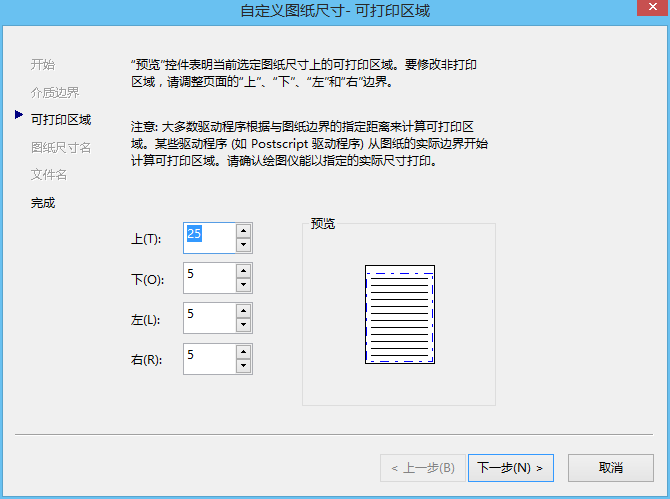
\includegraphics[scale=0.2]{kedayinqushezhi.png}}
\end{floatrow}
\end{figure}

\begin{lstlisting}
命令:pagesetup
\end{lstlisting}

\item 调整图纸空间的连接杆显示设置

首先,进入图纸空间中视口的模型空间。
\begin{lstlisting}
命令:mspace
\end{lstlisting}

其次,将视图方向切换为前视图方向。
\begin{lstlisting}
命令: -VIEW
输入选项 [?/删除(D)/正交(O)/恢复(R)/保存(S)/设置(E)/窗口(W)]: front
\end{lstlisting}
最后,将视口的显示比例设置为2:1,结果如图\ref{fig:lianjiegantuzhi1}所示。
\begin{figure}[htbp]
\centering
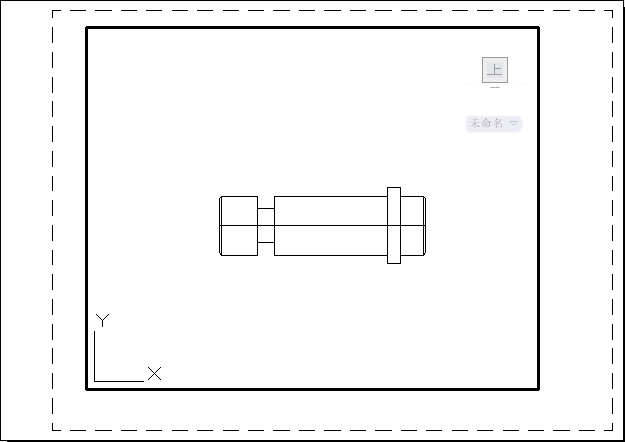
\includegraphics[scale=0.5]{lianjiegantuzhi1.png}
\caption{主视图显设置结果}\label{fig:lianjiegantuzhi1}
\end{figure}
\item 提取视图轮廓,并退出视口模型空间

调用轮廓命令提取视图的轮廓。
\begin{lstlisting}
命令: solprof
选择对象: 找到 1 个
选择对象:
是否在单独的图层中显示隐藏的轮廓线?[是(Y)/否(N)] <是>:
是否将轮廓线投影到平面?[是(Y)/否(N)] <是>:
是否删除相切的边? [是(Y)/否(N)] <是>:
\end{lstlisting}
接下来,退出视口模型空间
\begin{lstlisting}
命令: PSPACE
\end{lstlisting}
\item 修改图层设置

为保证显示正确的主视图,并方便尺寸标注和标题栏的绘制,需要调用图层管理器对图层做设置做以下修改。

\begin{enumerate}
\item 点击新建图层
\includegraphics[scale=0.6]{newlayer.png}图标,新建“标题栏”、“中心线”、“图框”和“尺寸标注”四个新图层。
\item 点击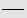
\includegraphics[scale=0.6]{linewidthselect.png}图标,将PV形状的图层和图框图层的线宽设置为0.5mm。
\item 点击“中心线”图层的线型设置图标
\includegraphics[scale=0.6]{linetypeselect.png},弹出图\ref{fig:linetypeset}所示的选择线型对话框,点击加载按钮,弹出图\ref{fig:loadlinetype}所示的加载或重载线型对话框,然后选择列表框中的CENTER线型并点击确定,返回选择线型对话框中,将CENTER线型选中,如图\ref{fig:selectcenterline}所示。最点击确定完成线型选择。
\item 将中心线图层设置为当前图层。
\end{enumerate}
\begin{lstlisting}
命令:layer
\end{lstlisting}
\begin{figure}[htbp]
\centering
\subfloat[]{\label{fig:linetypeset}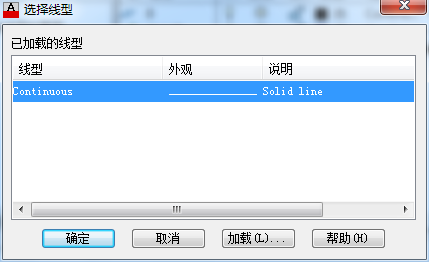
\includegraphics[scale=0.3]{linetypeset.png}}\hspace{20pt}
\subfloat[]{\label{fig:loadlinetype}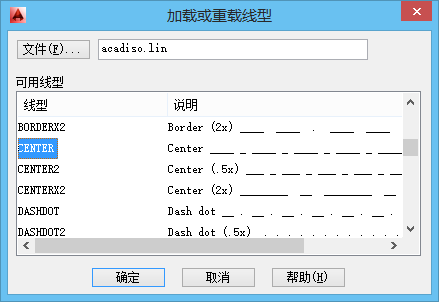
\includegraphics[scale=0.25]{loadlinetype.png}}\hspace{20pt}
\subfloat[]{\label{fig:selectcenterline}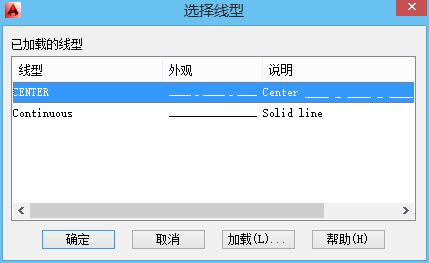
\includegraphics[scale=0.3]{selectcenterline.png}}
\caption{线型设置}
\end{figure}

修改改完成后的图层设置如图\ref{fig:lianjieganlayerset} 所示。
\begin{figure}[htbp]
\centering
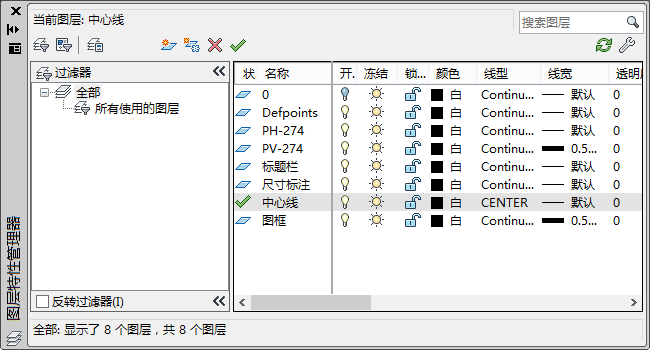
\includegraphics[scale=0.6]{lianjieganlayerset.png}
\caption{连接杆布局图层修改结果}\label{fig:lianjieganlayerset}
\end{figure}
\item 绘制中心线

由于连接杆是对称图形,视图生成后需要在图纸空间中手工绘制一条中线。因此在中心线图层设置为当前的状态下,可用直线命令来完成。AutoCAD中调用直线命令的方式有:
\begin{itemize}
\item 键盘输入line\index{line,直线} 或L。
\item 【绘图】$\rightarrow$【直线】。
\item 【绘图】$\triangleright$【直线】图标
\includegraphics[scale=0.5]{linetool.png}。
\end{itemize}

\begin{figure}[htbp]
\centering
\subfloat[]{\label{fig:centerlinedraw1}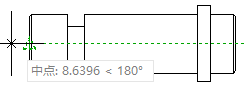
\includegraphics[scale=0.6]{centerlinedraw1.png}}\hspace{20pt}
\subfloat[]{\label{fig:centerlinedraw2}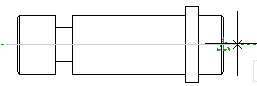
\includegraphics[scale=0.6]{centerlinedraw2.png}}\hspace{20pt}
\subfloat[]{\label{fig:centerlinedraw3}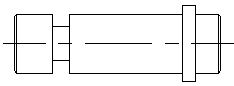
\includegraphics[scale=0.6]{centerlinedraw3.png}}
\caption{绘制中心线}
\end{figure}

\begin{lstlisting}
命令: line
指定第一个点:
\end{lstlisting}
调用直线命令后,命令示示指定第一个点,此时为保证中心线正好绘制在视图的中心,故采用对象捕捉追踪功能来完成第一点的指定,即先用鼠标捕捉到左端线的中心点,然后向左水平移动一小段距离单击鼠标左键指定第一点,如图\ref{fig:centerlinedraw1}所示。
\begin{lstlisting}
指定下一点或 [放弃(U)]:
\end{lstlisting}
命令提示指定下一点时,以指定第一点相同的方式绘定第二点,如图\ref{fig:centerlinedraw2}所示。
\begin{lstlisting}
指定下一点或 [放弃(U)]:
\end{lstlisting}
由于直线命令可以绘制多段直线,因此会继续提示指定下一点,此时用回车键结束命令,结果如图\ref{fig:centerlinedraw3}所示。
\end{procedure}
\subsection{制作图幅}
\begin{procedure}
\item 将当前图层设置为图框
\item 绘制图框

\begin{lstlisting}
命令: RECTANG
指定第一个角点或 [倒角(C)/标高(E)/圆角(F)/厚度(T)/宽度(W)]: 0,0
指定另一个角点或 [面积(A)/尺寸(D)/旋转(R)]: 267,200

命令: RECTANG
指定第一个角点或 [倒角(C)/标高(E)/圆角(F)/厚度(T)/宽度(W)]:
指定另一个角点或 [面积(A)/尺寸(D)/旋转(R)]: @-180,56
\end{lstlisting}
\end{procedure}
\subsection{制作标题栏}
\subsection{标注尺寸}
\endinput